\chapter{Fault handling and reconfiguration}
\subsection{Reaction Wheel Reconfiguration}
\todo{move reconfig part to fault isolation}
Fault isolation for the redundant reaction wheel configuration can be done by detecting which is the reaction wheel where the fault occurred and shutting it off and redistributing the torques to the rest of the reaction wheels. This reconfiguration can be represented by swapping the corresponding faulty columns to zero vectors. For example, if a fault occurs in the 3rd reaction wheel, the transformation matrix becomes $\underline{A}_{M,f3}$, as presented in equation \ref{eq:ReactFault}.

\begin{equation}
	\label{eq:ReactFault}
	\underline{A}_{M,f3} = \begin{bmatrix}
		\vec{Axis^{M}_{1}}       & \vec{Axis^{M}_{2}}   & \vec{0}   & \vec{Axis^{M}_{4}} 
	\end{bmatrix} 
\end{equation}

\begin{figure}[H]
	\centering 
	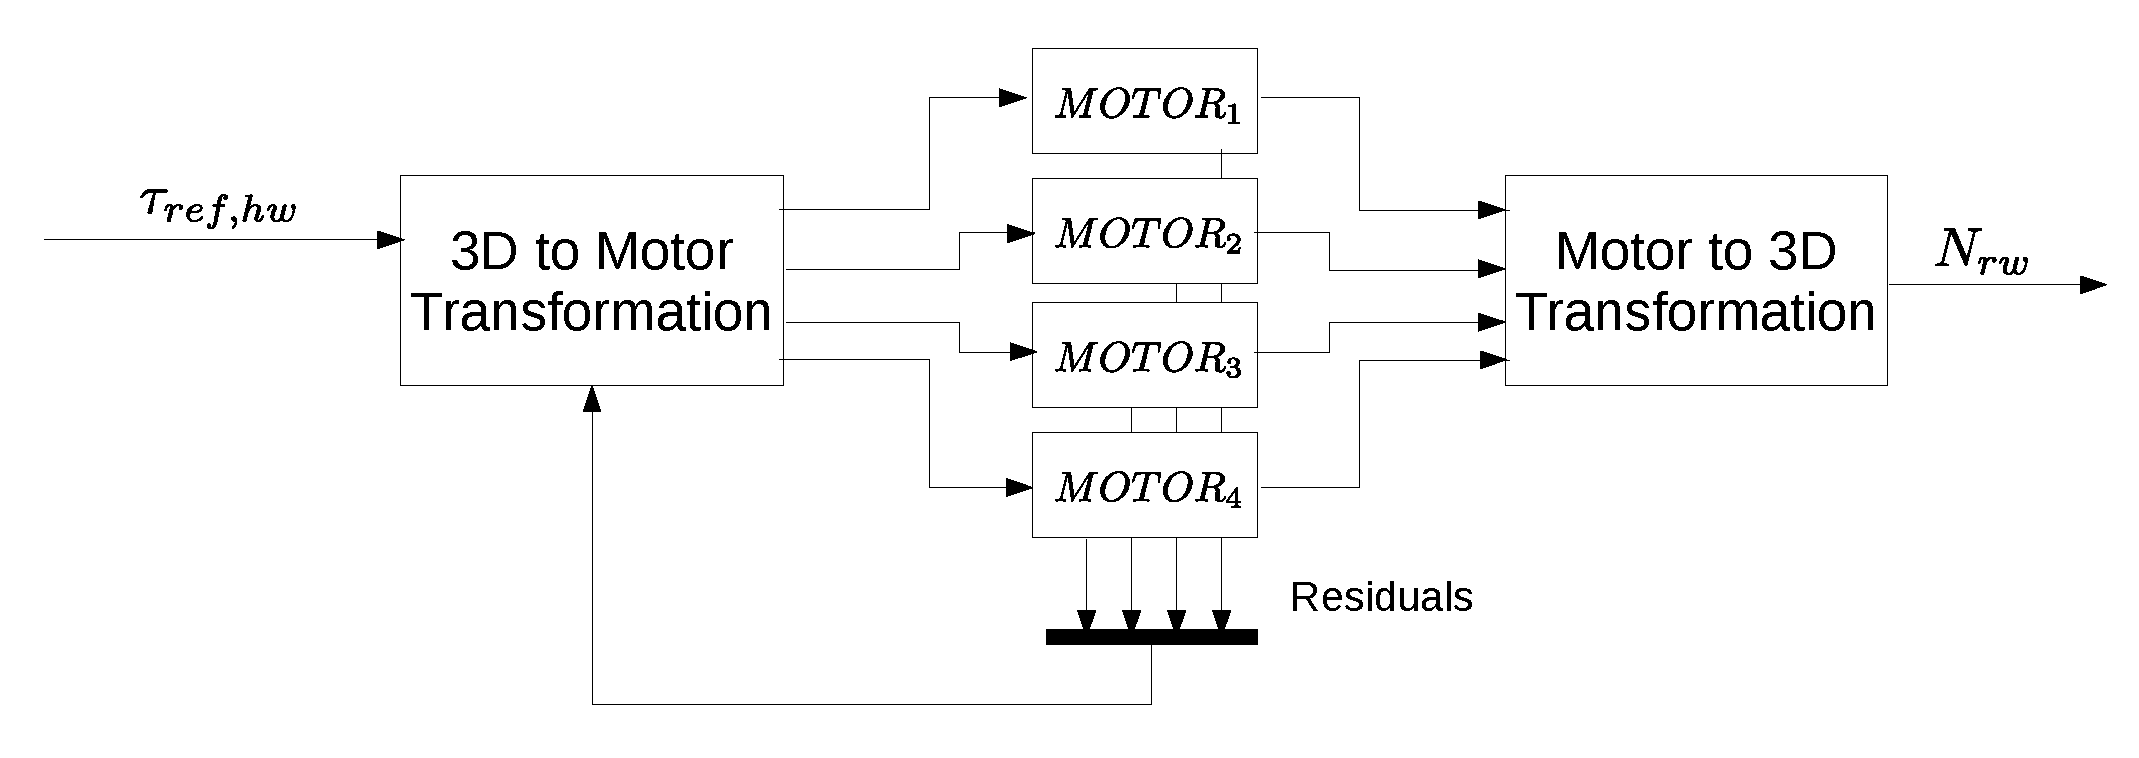
\includegraphics[width=170mm]{figures/reconfigure.pdf}	
	\caption{Reconfiguration Control Scheme for Reaction Wheels}
	\label{fig:reconfig}
\end{figure}

\nomenclature[S]{$\underline{A}_{M,fi}$}{Transformation matrix between axis oriented reaction wheel torque and torques in 3 dimensional body frame in case of faulty $i$th reaction wheel}

The pseudo inverse is calculated in the same manner as presented in equation \ref{eq:motorTrans}, as shown in equation \ref{eq:motorTransFault}. The torque distribution controller scheme which checks for faults in the motors, is presented in Figure \ref{fig:reconfig}

\begin{equation}
	\label{eq:motorTransFault}
	\underline{A}_{M,f3}^\dagger   = \underline{A}_{M,f3}^T  (\underline{A}_{M,f3} \underline{A}_{M,f3}^T)^{-1}
\end{equation}
%
%\begin{figure}
%	\centering
%	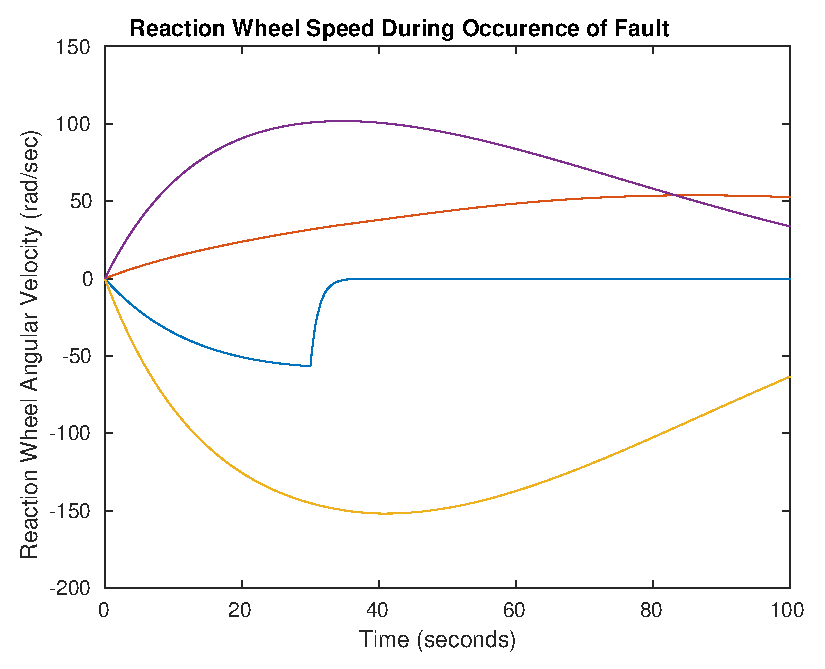
\includegraphics[width=120mm]{figures/residOmega}
%	\caption{Insert caption}
%	\label{fig:residualOmega}
%\end{figure} 

\subsubsection{Reconfiguration in case of residual fault detection}

\begin{figure}
	\centering
	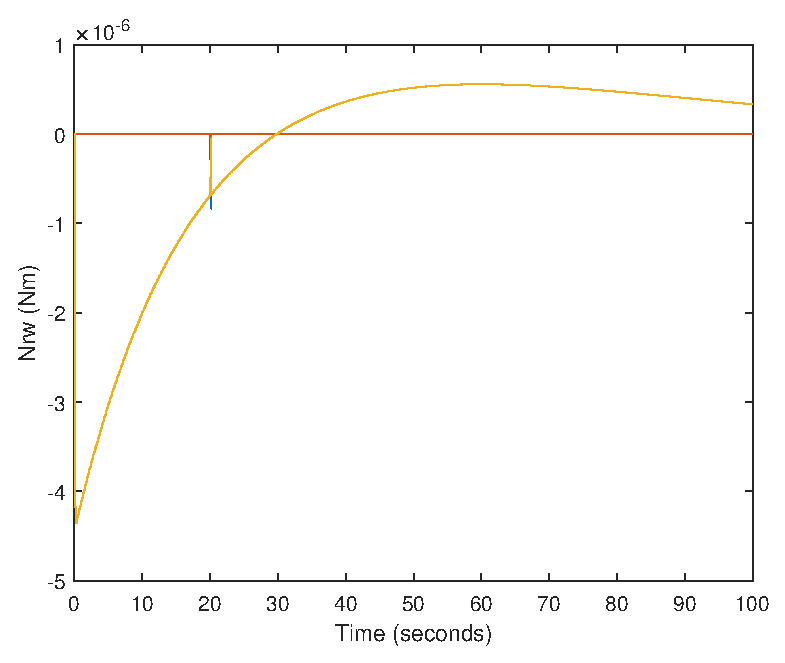
\includegraphics[width=120mm]{figures/3dTorque_resid_reconfig}
	\caption{$N_rw$ with fault occuring at 20 seconds}
\end{figure} 

\begin{figure}
	\centering
	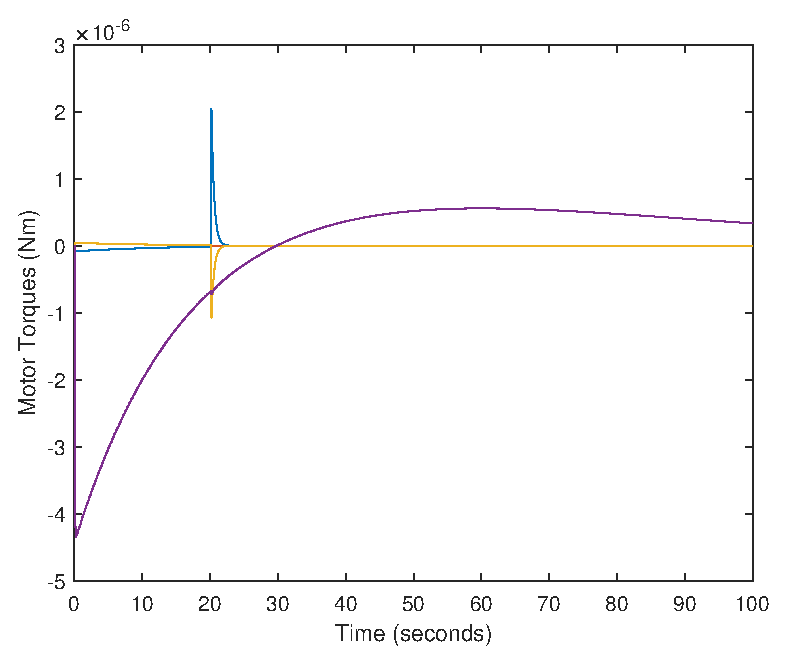
\includegraphics[width=120mm]{figures/torque_reconfig}
	\caption{$N_M$ with fault occuring at 20 seconds}
\end{figure} 

\begin{figure}
	\centering
	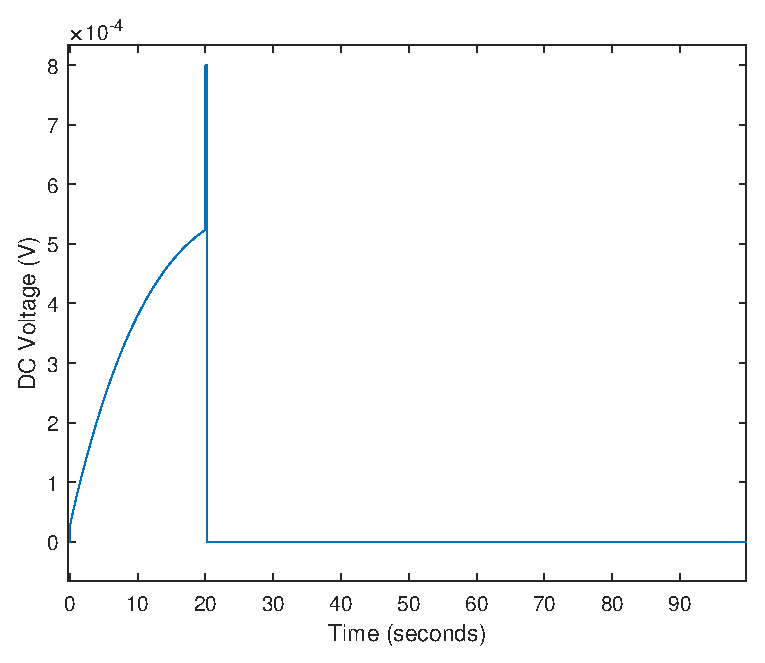
\includegraphics[width=120mm]{figures/voltage_reconfig}
	\caption{Voltage control signal with fault occuring at 20 seconds}
\end{figure} 


\begin{figure}
	\centering
	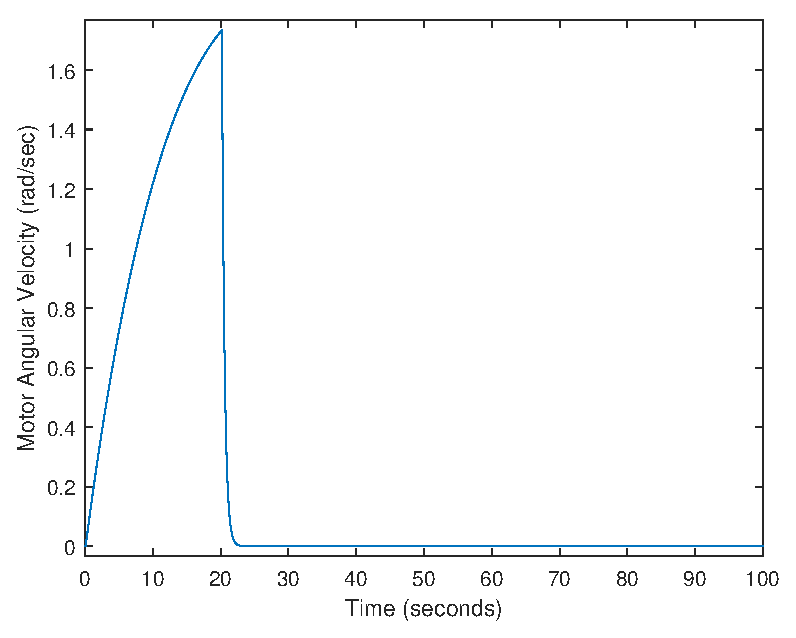
\includegraphics[width=120mm]{figures/omega_reconfig}
	\caption{$\omega_{M,i}$ with fault occuring at 20 seconds}
\end{figure} 


\begin{figure}
	\centering
	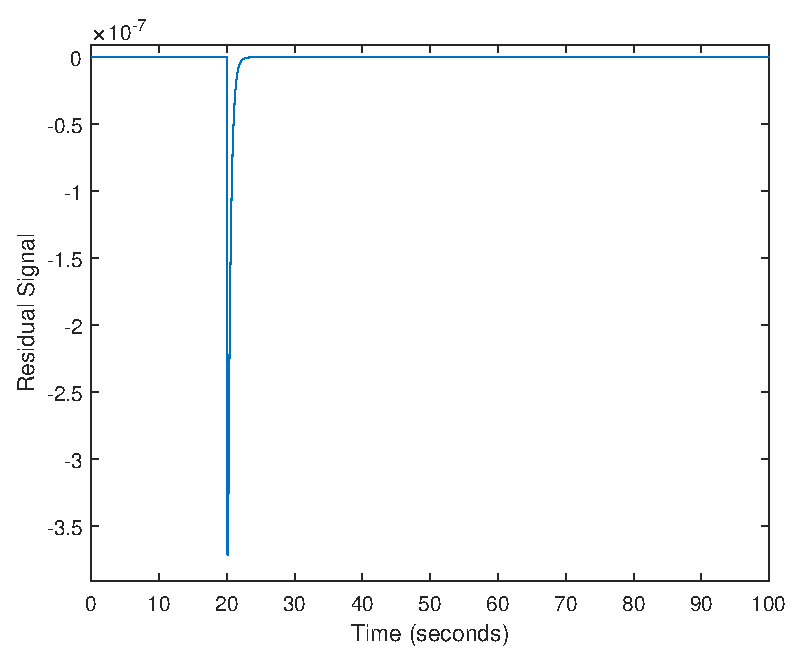
\includegraphics[width=120mm]{figures/residual_reconfig}
	\caption{Residual signal with fault occuring at 20 seconds}
\end{figure} 

\subsubsection{Reconfiguration in case of model-free sensor anomaly detection}

\begin{figure}
	\centering
	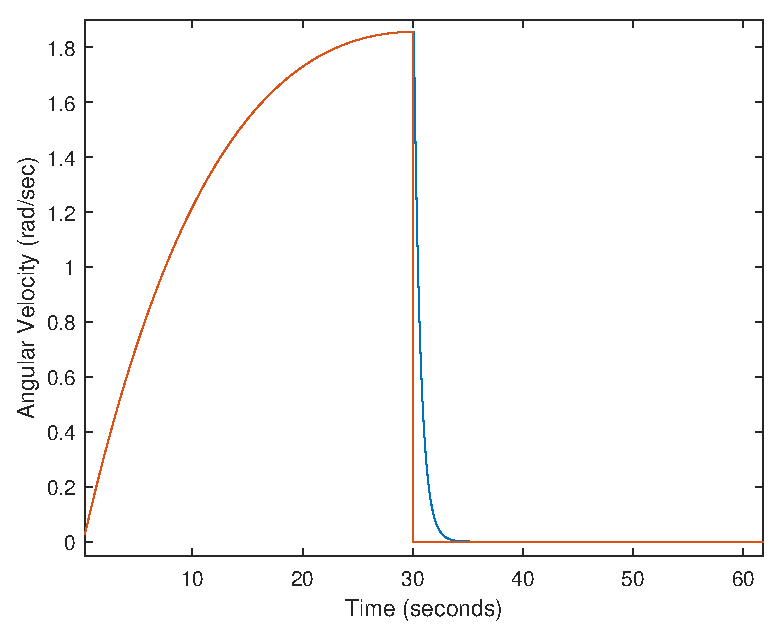
\includegraphics[width=120mm]{figures/omegaSensorfault_omega}
	\caption{$\omega_{M,i}$ sensor signal and actual value with fault occuring at 30 seconds}
\end{figure} 

\begin{figure}
	\centering
	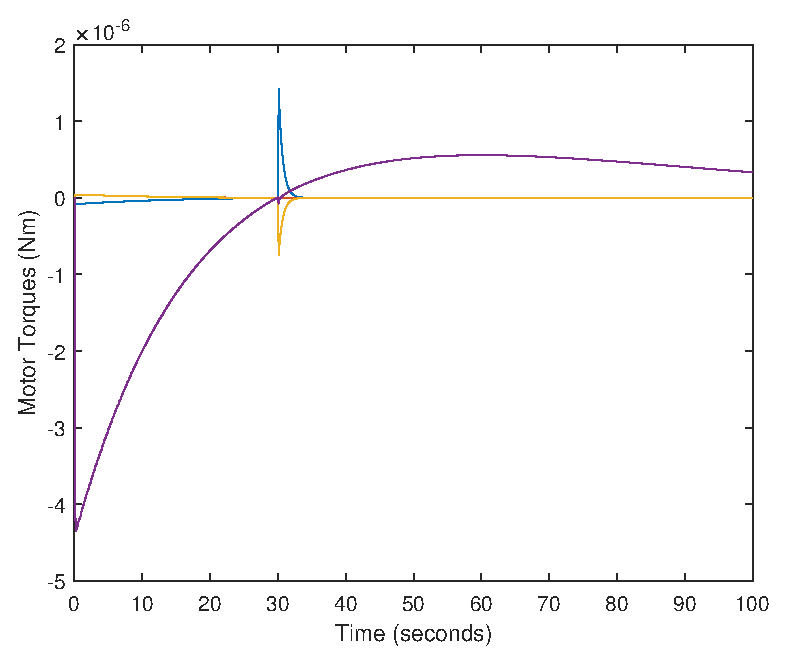
\includegraphics[width=120mm]{figures/omegaSensorfault_Nmotor}
	\caption{$N_M$ with $\omega$ sensor fault occuring at 20 seconds}
\end{figure} 

\begin{figure}
	\centering
	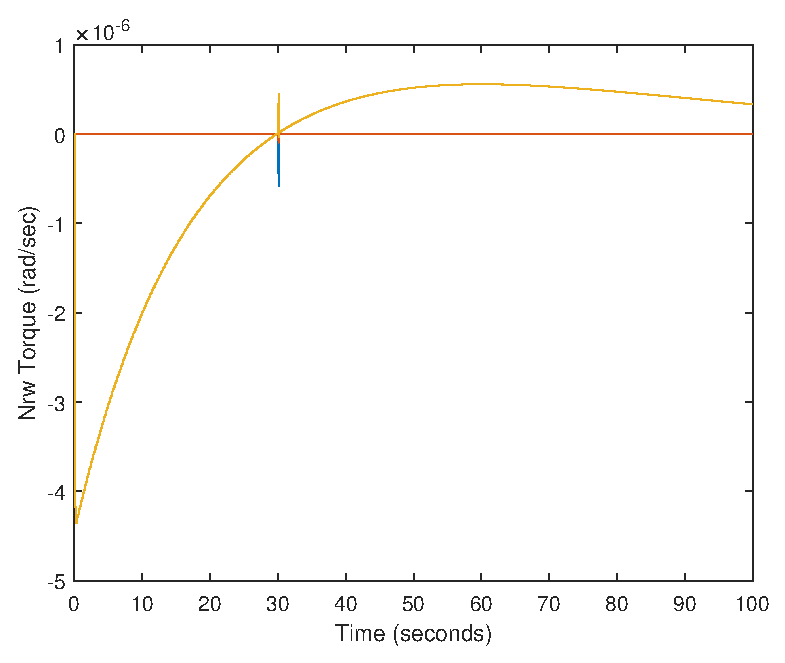
\includegraphics[width=120mm]{figures/omegaSensorfault_Nrw}
	\caption{$N_{rw}$ with $\omega$ sensor fault occuring at 20 seconds}
\end{figure} 
